\section{Auswertung}
\subsubsection{Versuchsteil A}
Bei der ersten Methode zur Bestimmung der Brennweite einer Linse wurden die Wertepaare für die Gegenstandsweite und Bildweite aus Tabelle \ref{tab:uno} aufgezeichnet.
Dabei wurden die Brennweiten nach Gleichung (2) aus den Werten berechnet.

\begin{table}[H]
    \begin{center}
      \caption{.Wertepaare der Gegenstandsweite $g$, der Bildweite $b$ und der berechneten Brennweite $f$}
      \label{tab:uno}
      \begin{tabular}{c|c|c} 
        \textbf{$g$ [cm]} & \textbf{$b$ [cm]} & \textbf{$f$ [cm]}\\
        \hline
        14.0 & 32.0 & 9.79 \\
        20.0 & 29.5 & 11.92 \\
        22.0 & 18.0 & 9.90 \\
        25.0 & 16.2 & 9.83 \\
        27.0 & 15.9 & 10.01 \\
        30.0 & 14.8 & 9.91 \\
        33.0 & 14.4 & 10.03 \\
        35.0 & 14.0 & 10.00 \\
        40.0 & 13.3 & 9.98 \\
        45.0 & 13.0 & 10.09
      \end{tabular}
    \end{center}
\end{table}

Aus den berechneten Brennweiten wird dann der Mittelwert und der dazugehörige Fehler nach
\begin{equation}
    \overline{x} = \frac{1}{N} \sum_{i=1}^N x_i \qquad \text{\&} \qquad \Delta \overline{x} = \sqrt{\frac{1}{N(N-1)}\sum \limits_{i=1}^N (x_i-\overline{x})^2}
\end{equation}
berechnet.

Für die Brennweite folgt also
\begin{equation}
    f_\text{Messung} = \SI{9.948 \pm 0.032}{cm}.     \notag
\end{equation}

Hinzufügend wird durch lineare Regression dieser Wert graphisch überprüft.
Dazu wird zu jedem Wertepaar eine Gerade nach
\begin{equation}
    y = m \cdot x + d \qquad \text{bzw.} \qquad  y = \left (\frac{b_i}{g_i}\right) \cdot x - b_i
\end{equation}
berechnet.
Dabei ist der negative Quotient aus $b$ und $g$ die Steigung der Geraden und $b$ der y-Achsenabschnitt.
In Abbildung \ref{fig:uno1} wird diese Gerade aufgetragen.
Des Weiteren soll aus dieser Abbildung die Brennweite abgelesen werden, indem der Schnittpunkt aller Geraden in der x-Koordinate und der y-Koordinate die Brennweite anzeigt.
Aus der näheren Ansicht in Abbildung \ref{fig:uno2} lässt sich dieser Schnittpunkt nicht genau identifizieren.
Es ergibt sich für die abgelesene Brennweite

\begin{equation}
    f_\text{Graph} \approx \SI{9.45 \pm 0.5}{cm}     \notag
\end{equation}.

\begin{figure}[h]
    \centering
    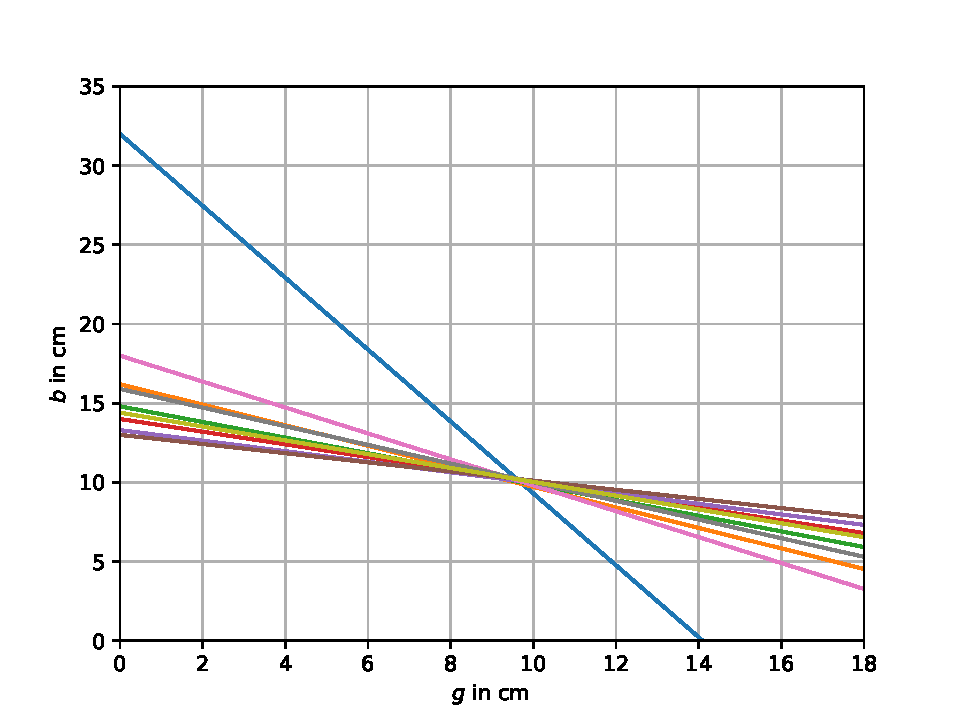
\includegraphics[height=6cm]{Auswertung/Uno1.pdf}
    \caption{Geradenkonstruktion von Bild- und Gegenstandsweite.}
    \label{fig:uno1}
\end{figure}

\begin{figure}[h]
    \centering
    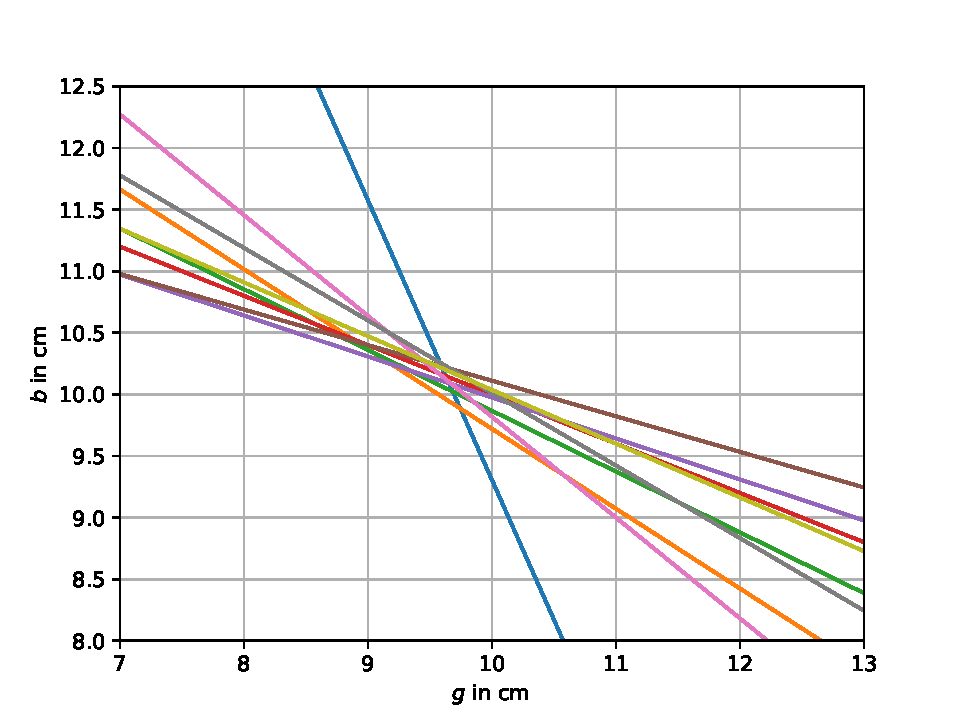
\includegraphics[height=6cm]{Auswertung/Uno2.pdf}
    \caption{Nähere Ansicht der Geradenkonstruktion von Bild- und Gegenstandsweite.}
    \label{fig:uno2}
\end{figure}

\subsection{Versuchsteil B - Bessel}
Bei der Methode von Bessel wurden zunächst die Gegenstandsweiten und Bildweiten gemessen und daraus dann die Abstände $e$ und $d$ nach
\begin{equation}
    e = g_1 + b_1 = g_2 + b_2 \qquad \text{\&} \qquad d = g_1 - b_1 = g_2 - b_2
\end{equation}
berechnet.
Dabei wird $d$ einerseits durch $g_1 - b_1$ und andererseits nach $g_2 - b_2$ bestimmt und daraus der Mittelwert nach Gleichung (7) berechnet.
Der dazugeörige Fehler wird nach der Gaußschen Fehlerfortpflanzung für $i \in \{1,2\}$
\begin{equation}
    \label{eqn:Gauss}
    \Delta d = \sqrt{\left ( \frac{\partial d}{\partial g_i} \Delta g_i \right )^2 + \left ( \frac{\partial d}{\partial i} \Delta b_i \right )^2} 
\end{equation}
In der Tabelle \ref{tab:dos} sind die Werte für weißes Licht mit der berechneten Brennweite nach Gleichung (4) aufgetragen.

\begin{table}[H]
    \begin{center}
      \caption{.Wertepaare von $e$, $d$ und der berechneten Brennweite $f$ bei weißem Licht}
      \label{tab:dos}
      \begin{tabular}{c|c|c} 
        \textbf{$e$ [cm]} & \textbf{$d$ [cm]} & \textbf{$f$ [cm]}\\
        \hline
        75.0 & 51.4 & 9.94 \\
        70.0 & 46.1 & 9.91 \\
        65.0 & 40.6 & 9.91 \\
        80.0 & 56.7 & 9.95 \\
        60.0 & 34.8 & 9.95 \\
        55.0 & 29.2 & 9.99 \\
        50.0 & 22.8 & 9.99 \\
        45.0 & 15.2 & 9.97 \\
        67.0 & 42.8 & 9.92
      \end{tabular}
    \end{center}
\end{table}

Nach Gleichung (7) ergibt sich für den Mittelwert der Brennweite bei weißem Licht mit entsprechendem Fehler
\begin{equation}
    f_\text{wei\ss{}} = \SI{9.925 \pm 0.010}{cm}.     \notag
\end{equation}

Dieser Versuch wurde für rotes und blaues Licht wiederholt um die chromatische Abberation zu überprüfen.
Dabei wurden die Messwerte aus Tabelle \ref{tab:farbe} aufgezeichnte.
FÜr die Größe $d$ wird jeweils wieder der Mittelwert nach Gleichung (7) und der Fehler nach Gleichung \ref{eqn:Gauss} berechnet.

\begin{table}[H]
    \begin{center}
      \caption{.Wertepaare von $e$, $d$ und der berechneten Brennweite $f$ bei rotem und blauem Licht}
      \label{tab:farbe}
      \begin{tabular}{c|c|c||c|c|c} 
        \textbf{$e_\text{rot}$ [cm]} & \textbf{$d_\text{rot}$ [cm]} & \textbf{$f_\text{rot}$ [cm]} & \textbf{$e_\text{blau}$ [cm]} & \textbf{$d_\text{blau}$ [cm]} & \textbf{$f_\text{blau}$ [cm]}\\
        \hline
        70.0 & 45.9 & 9.98 & 70.0 & 46.2 & 9.88 \\
        65.0 & 40.0 & 10.10 & 65.0 & 40.5 & 9.94 \\
        60.0 & 34.4 & 10.07 & 60.0 & 34.9 & 9.93 \\
        55.0 & 28.4 & 10.08 & 55.0 & 28.9 & 9.95 \\
        50.0 & 22.4 & 9.99 & 50.0 & 32.8 & 9.90
      \end{tabular}
    \end{center}
\end{table}

Ebenfalls nach Gleichung (4) und (7) ergibt sich für die beiden Brennweiten für rotes und blaues Licht
\begin{equation}
    f_\text{rot} = \SI{10.043 \pm 0.025}{cm} \qquad \text{\&} \qquad f_\text{blau} = \SI{9.920 \pm 0.014}{cm}.    \notag
\end{equation}

\subsection{Versuchsteil C - Abbe}
Im letzten Versuchsteil wurde die Methode von Abbe verwendet.
Dazu wurde aufgrund der Nutzung zweier hintereinanderstehenden Linsen die Größen $g'$ und $b'$, wie in Abbildung \ref{fig:Aufbau3} beschrieben, definiert.
Des Weiteren wurden neben der Bild- und Gegenstandsweite zusätzlich die Größe des Bildes gemessen.
Bei einer konstanten Gegenstandsgröße von $G = \SI{3}{cm}$ wurden die Werte aus Tabelle \ref{tab:tres} gemessen.

\begin{table}[H]
    \begin{center}
      \caption{.}
      \label{tab:tres}
      \begin{tabular}{c|c|c|c|c} 
        \textbf{$g'$ [cm]} & \textbf{$b'$ [cm]} & \textbf{$V$} & \textbf{$1 + \frac{1}{V}$} & \textbf{$1 + V$}\\
        \hline
        20.0 & 69.2 & 1.9 & 1.53 & 2.90 \\
        25.0 & 55.9 & 1.2 & 1.83 & 2.20 \\
        30.0 & 49.9 & 0.9 & 2.11 & 1.90 \\
        35.0 & 45.9 & 0.7 & 2.43 & 1.70 \\
        40.0 & 43.5 & 0.6 & 2.67 & 1.60 \\
        32.5 & 47.5 & 0.8 & 2.30 & 1.77 \\
        27.5 & 52.0 & 1.0 & 2.00 & 2.00 \\
        37.5 & 47.0 & 0.6 & 2.67 & 1.60
      \end{tabular}
    \end{center}
  \end{table}

Mit Hilfe der linearen Regression nach Gleichung (5) und (6) ergeben sich die Abbildungen \ref{fig:abbe1} und \ref{fig:abbe2}.
Die berechnete Steigung der Graphen ergibt also die Brennweite des Linsenpaares.
Es ergeben sich für die Brennweite also zwei unterschiedliche Werte, einerseits beim Auftragen von $g'$ gegen $1+\frac{1}{V}$ und andererseits beim Auftragen von $b'$ gegen $1+V$.
\begin{equation}
    f_g = \SI{16.484 \pm 0.501}{cm}  \qquad \text{\&} \qquad h' = \SI{5.198 \pm 2.521}{cm} \\ 
    f_b = \SI{18.723 \pm 0.954}{cm}  \qquad \text{\&} \qquad h = \SI{14.697 \pm 3.816}{cm}  \notag
\end{equation}

Nach Gleichung (7) ergibt sich also für den Mittelwert der Brennweite
\begin{equation}
    f = \SI{17.604 \pm 3.422}{cm}  \notag
\end{equation}.

\begin{figure}[h]
    \centering
    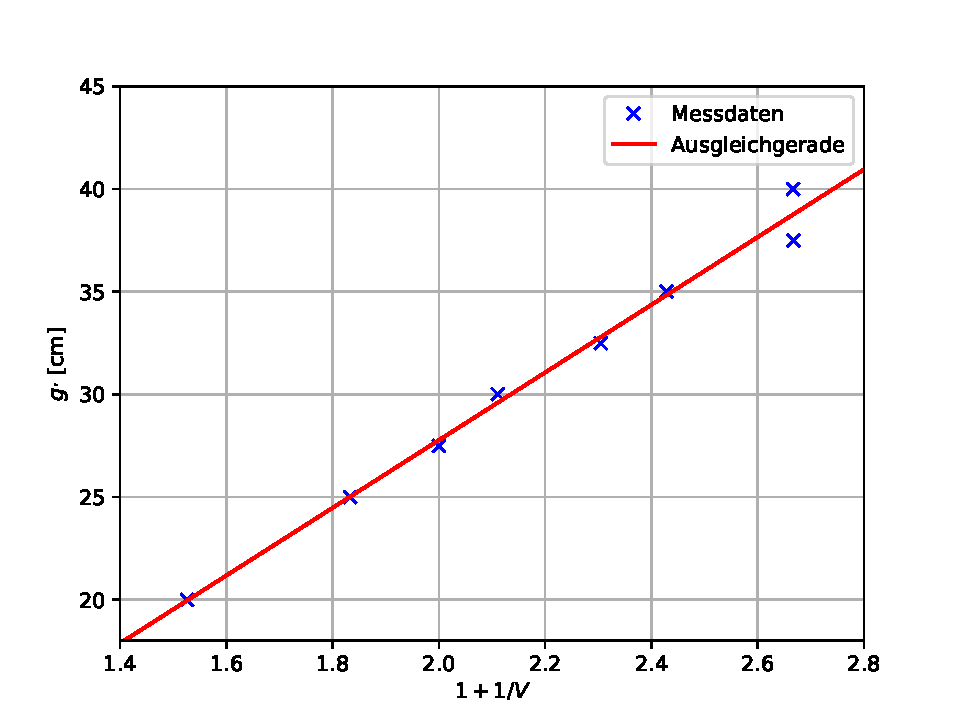
\includegraphics[height=6cm]{Auswertung/Abbe1.pdf}
    \caption{Auftragung von $g'$ gegen $1+\frac{1}{V}$.}
    \label{fig:abbe1}
\end{figure}
\begin{figure}[h]
    \centering
    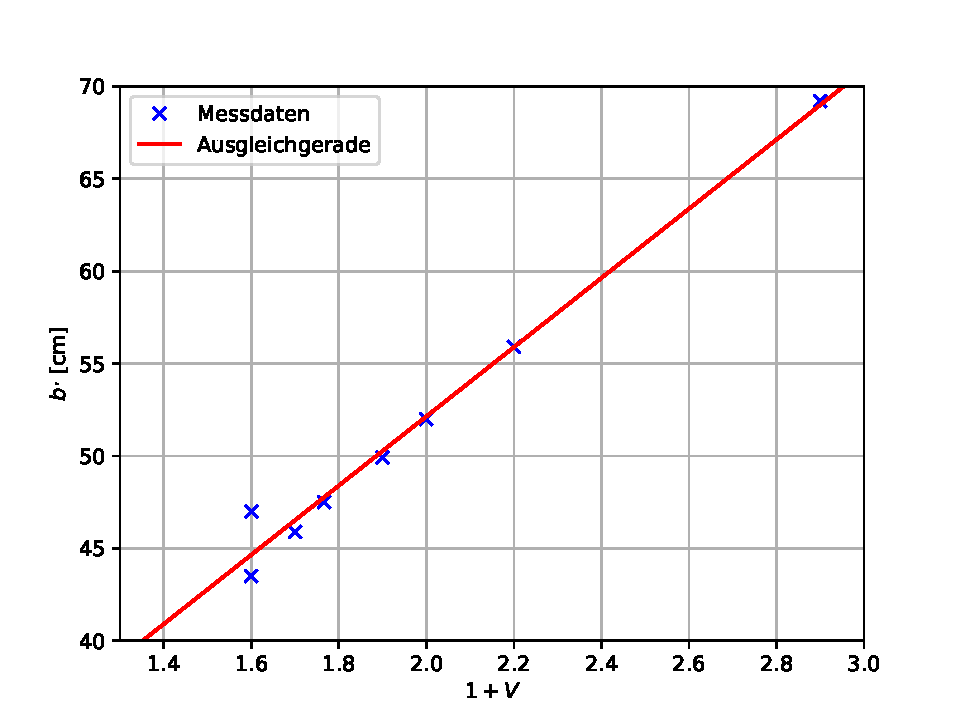
\includegraphics[height=6cm]{Auswertung/Abbe2.pdf}
    \caption{Auftragung von $b'$ gegen $1+V$.}
    \label{fig:abbe2}
\end{figure}
